% A good introduction to latex can be found here:
%  http://www.cse.ohio-state.edu/~hank/latex/lshort141.pdf

\documentclass{article}
\usepackage{amsmath}

\usepackage{full page}  % make the margins somewhat smaller than the default

\usepackage{listings}  %  needed for source code listings
\usepackage{color}
\usepackage{hyperref}
\usepackage{graphicx}
\usepackage[tight,footnotesize]{subfigure}

\definecolor{javared}{rgb}{0.7,0,0} % for strings
\definecolor{javagreen}{rgb}{0.25,0.6,0.35} % comments
\definecolor{javapurple}{rgb}{0.55,0,0.40} % keywords
\definecolor{javadocblue}{rgb}{0.25,0.35,0.85} % javadoc
 
\lstset{language=Java,
basicstyle=\ttfamily,
keywordstyle=\color{javapurple}\bfseries,
stringstyle=\color{javared},
commentstyle=\color{javagreen},
morecomment=[s][\color{javadocblue}]{/**}{*/},
numbers=left,
numberstyle=\tiny\color{black},
stepnumber=2,
numbersep=10pt,
tabsize=4,
showspaces=false,
showstringspaces=false,
frame=shadowbox,
numbers=left
} 

% set the document title, author, and date here.
%  once set, the \maketitle command (within the document)
%  will display them nicely
\title{Motion Planning}
\author{Junjie Guan $<gjj@cs.dartmouth.edu>$}

\begin{document}
\maketitle

\tableofcontents

\section{Introduction}

Motion planning is a very intersting problem in our realworld. One key issue here is that the metrics beacome infinite in real world, while computer can only handle finite number of states. In this report we introduce some planning methods that is able to build a search tree/graph for real world problem (here the problem is motion planning).













\clearpage
\section{Probabilistic Roadmap (PRM)}
\subsection{Basic Idea}

The basic idea of PRM is first sampling the real world and creat a finite configuration space. Then we create a search graph based on the relationship of each configuration (usually a multi-dimensional distance). Then we use traditional path searching algorithm such as A* to find a solution from the start to the goal.

\begin{figure*}[!h]
\centering
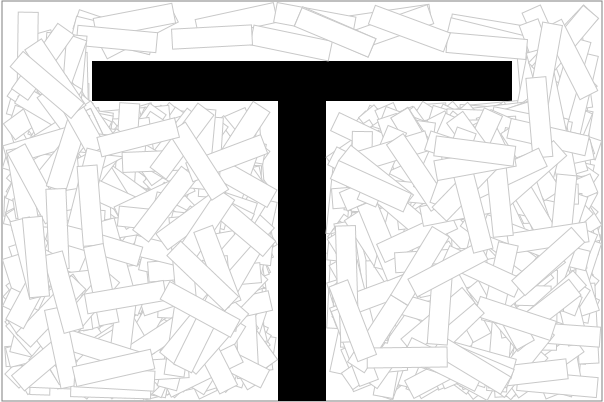
\includegraphics[width=0.927\textwidth]{sample.png}
\caption{A demostration of A* algorithm}
\label{sampling}
\end{figure*}

Figure \ref{sampling} demostrate a sampling space, with all the random configuration of a two-links robot arm (gray rectagnle). The black area is the obstable in the space. 

\subsection{Discussions}
In this homework, in the sampling phase, an intuitive way is to randomly generate the configuration, and check whether it is a legal configuration. If not, dismiss it and keep generate another until a valid one occurs. 

An issue we should concern about is, this method usually generate more configuration in a relatively large free space (in motion planning, meaning a space with a few obtacles ). This would likely lead to a result that there are not enough configurations in the tricky space (such as a narrow corridor when referring to motion planning problem).

If you look at the figure \ref{sampling}, you will observe that there are significantly less configurations on the top because it is not easy to generat a legal configuration there. 

Concerning this issue, we can propose some better sampling method.  A simple idea is, every time when we detect a sampling collision, instead of simply dismiss it, we try to move the configuration in a random direction direction until it reaches the edge of the obstacles -- becoming a legal configuration. By doing so, we can make the density of narrow space higher than the normal open space, so that the computer can handle the corner case much better.



\subsection{Code implementation}


\subsubsection{constructor}

\textbf{RoadMapProblem} constructor gives you an outline of building the road map.

\begin{lstlisting}[numbers=left]
public RoadMapProblem(World m, Double[] config1, Double[] config2,
    int density, int K) {
  // initiate the basic parameters 
  k_neighbour = K;
  map = m;
  startArm = new ArmRobot(config1);
  goalArm = new ArmRobot(config2);
  startNode = new RoadMapNode(startArm, 0.);
  // start sampling and generating the roadmap
  getSampling(density);
  getConnected();
}
\end{lstlisting}


\subsubsection{getSampling}

\textbf{getSampling} is used to create the sample configurations, preparing for roadmap generation.

\textbf{Line 3:} Generate the random configuration.
\textbf{Line 5:} Check if the newly created configuration is legal. Noted that I modify the the armCollision function, so that the configuration will be confined into the world space.
\textbf{Line 6:} Add the new configuration to the hash set.

\begin{lstlisting}[numbers=left]
public void getSampling(int density) {
  while (density > 0) {
    Double[] rConfig = getRandCfg(startArm.links, map);
    ArmRobot toBeAdded = new ArmRobot(rConfig);
    if (!map.armCollision(toBeAdded)) {
      samplings.add(toBeAdded);
      density--;
    }
  }
}
\end{lstlisting}

\subsubsection{getRandCfg}

\textbf{getRandCfg} is used to generate the new random configuration.

\textbf{Line 3:} noted that the length or each arm is fixed.

\begin{lstlisting}[numbers=left]
private Double[] getRandCfg(int num, World map) {
  Random rd = new Random();
  Double[] cfg = new Double[2 * num + 2];
  // randomize the start position
  cfg[0] = rd.nextDouble() * map.getW();
  cfg[1] = rd.nextDouble() * map.getH();
  // System.out.println(cfg[0]/map.getW() + "," + cfg[1]/map.getH());
  for (int i = 1; i <= num; i++) {
    // the length of each arm remains the same
    cfg[2 * i] = startArm.config[2 * i];
    // randomize the angle
    cfg[2 * i + 1] = rd.nextDouble() * Math.PI * 2;
  }
  return cfg;
}
\end{lstlisting}

\subsubsection{getConnected}

\textbf{getConnected} is used to connect the sampling. Basic idea is iterating through the samples and connect to $k$ nearest vertice in the roadmap. The raodmap is implemented in adjacent linked list style.

\begin{lstlisting}[numbers=left]
public void getConnected() {
  // initiate the connecting with start arm
  ArmLocalPlanner ap = new ArmLocalPlanner();
  PriorityQueue<AdjacentCfg> tmpq;
  for (ArmRobot ar : samplings)
    roadmap.put(ar, new PriorityQueue<AdjacentCfg>());

  // add the start and goal to the roadmap
  connected.add(startArm);
  connected.add(goalArm);
  for (ArmRobot ar : samplings) {
    for (ArmRobot arOther : connected) {
      if (ar != arOther
          && !map.armCollisionPath(ar, ar.config, arOther.config)) {
        Double dis = ap.moveInParallel(ar.config, arOther.config);
        roadmap.get(ar).add(new AdjacentCfg(arOther, dis));
        // make sure the configuration only points to k nearest neighbour
        if (roadmap.get(ar).size() > k_neighbour)
          roadmap.get(ar).poll();
        // make sure that it an undirected graph
        roadmap.get(arOther).add(new AdjacentCfg(ar, dis));
        if(roadmap.get(arOther).size() > k_neighbour)
          roadmap.get(arOther).poll();
      }
    }
    // keep track of the connected configurations
    connected.add(ar);
  }
}
\end{lstlisting}




\subsubsection{boundary detect}
\textbf{boundary detect} makes sure that the configuration do not escape the world area.

\begin{lstlisting}[numbers=left]
...
for (int j = 1; j <= p.getLinks(); j++) {
  link_i = p.getLinkBox(j);
  for(int i = 0; i < link_i.length; i++){
  if(link_i[i][0] < 0 || link_i[i][0] > window_width)
    return true;
  if(link_i[i][1] < 0 || link_i[i][1] > window_height)
    return true;
  }
}
...
\end{lstlisting}




\subsection{Output demonstration}
Figure \ref{startendrmp} demostrates the start and and end configuration of my testing. Figure \ref{1-0}-\ref{1-2} presents 3 examples of the testing case, with increasing sampling difficulty. The number of sample configuration is 500, and $k$ is 15.
\begin{figure*}[!h]
\centering
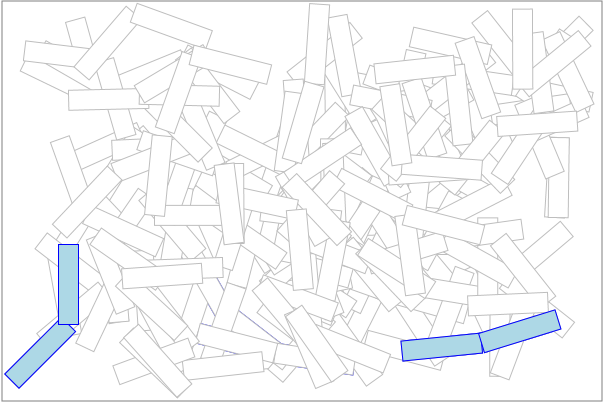
\includegraphics[width=0.827\textwidth]{0-1.png}
\caption{start and end of testing}
\label{startendrmp}
\end{figure*}

\begin{figure*}[!h]
\centering
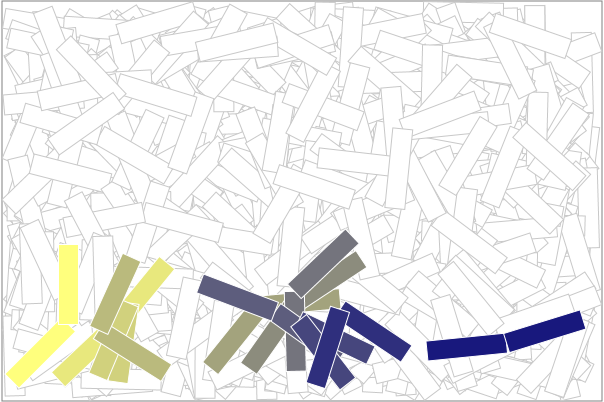
\includegraphics[width=0.827\textwidth]{1-0.png}
\caption{test in empty space}
\label{1-0}
\end{figure*}

\begin{figure*}[!h]
\centering
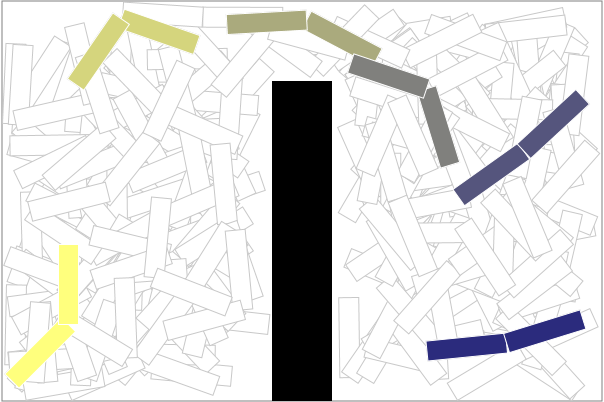
\includegraphics[width=0.827\textwidth]{1-1.png}
\caption{test with an obstacle.}
\label{1-1}
\end{figure*}

\begin{figure*}[!h]
\centering
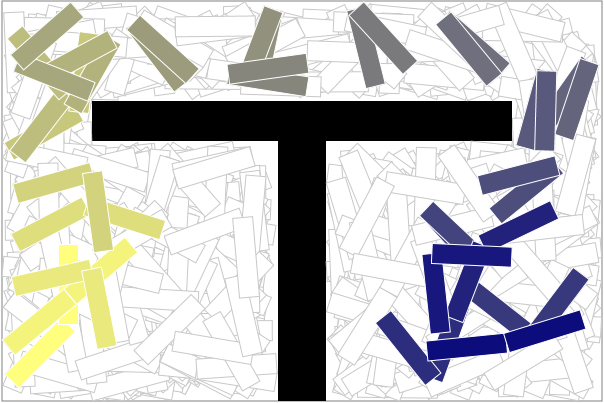
\includegraphics[width=0.827\textwidth]{1-2.png}
\caption{test with corridor. The movement becomes more tricky and complex}
\label{1-2}
\end{figure*}






\clearpage
\section{Rapidly Exploring Random Tree}
\subsection{Basic Idea}
The basic idea of RRT is to grow a tree from the start, to fill up the infinite or over complex space. The most simple and intuitive way is to randomly generate legal configuration, and grow the tree towards the configuration. 





\subsection{Code implementation}


\subsubsection{growTree2Goal}

\textbf{growTree2Goal} keeps interatively expanding the tree until one of the node close to the goal. (I think the code is already quite self-explanatory, no further introduction is needed) 

\begin{lstlisting}[numbers=left]
public void growTree2Goal(int num4grow) {
  while (num4grow > 0) {
    // generate new random car
    CarRobot newRandCar = new CarRobot(getRandCfg(map));
    // if the car is valid
    if (!map.carCollision(newRandCar)) {
      CarRobot nearest = findNearestInTree(newRandCar);
      CarRobot newAdded = expandTree(newRandCar, nearest);
      if(!connected.contains(newAdded)) {
        addNewNode2Tree(newAdded, nearest);
        // terminate the iteration if reaching the goal
        if (newAdded.getDistance(goalCar) < 20) {
          addNewNode2Tree(goalCar, newAdded);
          break;
        }
        num4grow--;
      }
    }
  }
}
\end{lstlisting}

\textbf{findNearestInTree} finds the vertex that is nearest to the new randomly generated node.

\begin{lstlisting}[numbers=left]
private CarRobot findNearestInTree(CarRobot newRandCar) {
  Double minDis = Double.MAX_VALUE;
  CarRobot nearest = null;
  for (CarRobot cr : connected) {
    double dis = newRandCar.getDistance(cr);
    if (minDis > dis) {
      minDis = dis;
      nearest = cr;
    }
  }
  return nearest;
}
\end{lstlisting}

\textbf{expandTree} trys to expand to 6 different directions, and return the expansion that is nearest to the randomly generated node.

\begin{lstlisting}[numbers=left]
private CarRobot expandTree(CarRobot newRandCar, CarRobot nearest) {
  // initiate the auxiliary object
  Double minDis = Double.MAX_VALUE;
  SteeredCar sc = new SteeredCar();
  CarRobot newAdded = null, newCarRobot = new CarRobot();
  // try to expand to 6 different directions
  for (int i = 0; i <= 5; i++) {
    newCarRobot = new CarRobot(sc.move(nearest.getCarState(), i, 1.));
    // System.out.println("newCarRobot: " + newCarRobot);
    if (!map.carCollision(newCarRobot)) {
      double dis = newCarRobot.getDistance(newRandCar);
      if (minDis > dis) {
        minDis = dis;
        newAdded = newCarRobot;
      }
    }
  }
  return newAdded;
}

\end{lstlisting}

\textbf{addNewNode2Tree} trys to expand to 6 different directions, and return the expansion that is nearest to the randomly generated node.

\begin{lstlisting}[numbers=left]
private void addNewNode2Tree(CarRobot newNode, CarRobot parentNode) {
  connected.add(newNode);
  RRTree.get(parentNode).add(new AdjacentCfg(newNode, 1));
  RRTree.put(newNode, new HashSet<AdjacentCfg>());
}
\end{lstlisting}





\subsubsection{getSuccessors}

\textbf{getSuccessors} is pretty simple. Simply return the children nodes in the exploring tree.

\begin{lstlisting}[numbers=left]
public ArrayList<SearchNode> getSuccessors() {
  ArrayList<SearchNode> successors = new ArrayList<SearchNode>();
  for (AdjacentCfg adj : RRTree.get(car)) {
    successors.add(new RRTnode(adj.ar, adj.dis + cost));
  }
  return successors;
}
\end{lstlisting}











\subsection{Output demonstration}
Figure \ref{2-1}-\ref{2-3} presents 3 examples of the testing case, with increasing sampling difficulty. From the last two case we can observe that, the tree on left part is much more complicate. This is because the left part has keep randomly generating the tree when one of the branch trying to explore through the corridor. I think using a bidirectional spaning can cut the expense of exploring corridor to half.

\begin{figure*}[!h]
\centering
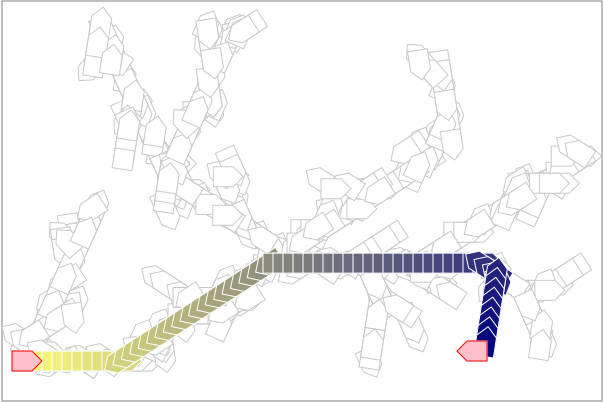
\includegraphics[width=0.827\textwidth]{2-1.png}
\caption{test in empty space}
\label{2-1}
\end{figure*}

\begin{figure*}[!h]
\centering
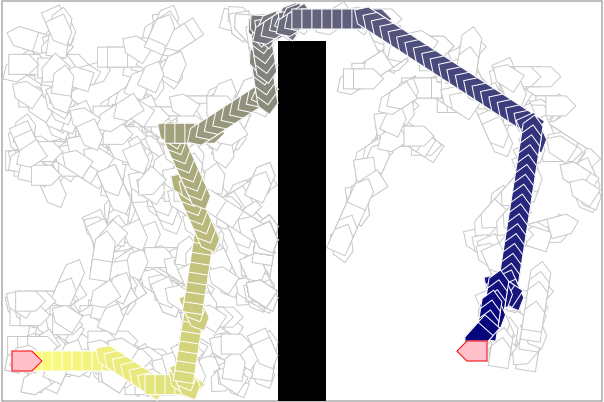
\includegraphics[width=0.827\textwidth]{2-2.png}
\caption{test with an obstacle.}
\label{2-2}
\end{figure*}

\begin{figure*}[!h]
\centering
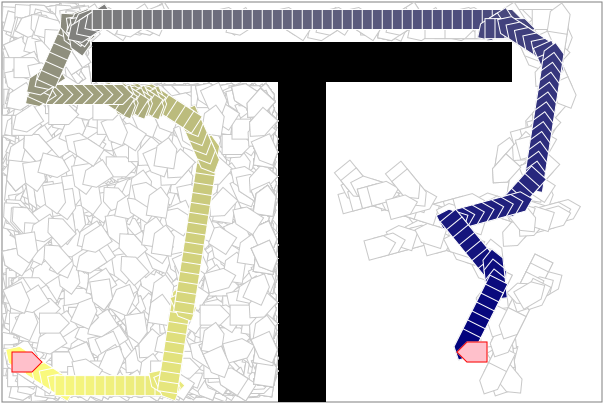
\includegraphics[width=0.827\textwidth]{2-3.png}
\caption{test with corridor. The movement becomes more tricky and complex}
\label{2-3}
\end{figure*}






\subsection{Extension: bidirectional search}







\section{Previous Work}



\end{document}